\documentclass[12pt]{article}

\usepackage[margin=1in]{geometry}
\usepackage{amsmath,amsthm,amssymb}
\usepackage{mathtools}
\usepackage{mathrsfs}
\usepackage{enumitem}
\usepackage{physics}

\usepackage{tikz}
\usetikzlibrary{calc,decorations.markings,patterns}

\newcommand{\magsq}[1]{\big|#1\big|^2}
\newcommand{\avg}[1]{\left<#1\right>}
\newcommand{\fullint}{\int_{-\infty}^\infty}
\newcommand{\fullintd}[1]{\fullint\dd#1\:}
\newcommand{\cint}[2]{\int_{#1}^{#2}}
\newcommand{\cintd}[3]{\cint{#1}{#2}\dd#3\:}

\def\firstcircle{(90:.75cm) circle (1cm)}
\def\secondcircle{(210:.75cm) circle (1cm)}
\def\thirdcircle{(330:.75cm) circle (1cm)}

\begin{document}

\title{610 Notes Tikz Pictures}
\author{Sean Ericson \\ Phys 610}
\maketitle

\section*{Reference Pics}

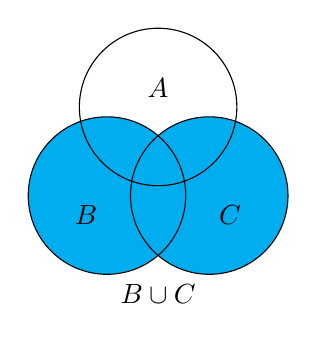
\begin{tikzpicture}
    \fill[cyan] \thirdcircle;
    \fill[cyan] \secondcircle;
    \draw \firstcircle node[text=black,above] {$A$};
    \draw \secondcircle node [text=black,below left] {$B$};
    \draw \thirdcircle node [text=black,below right] {$C$};
    \node[below] at (current bounding box.south) {$B \cup C$};
\end{tikzpicture}

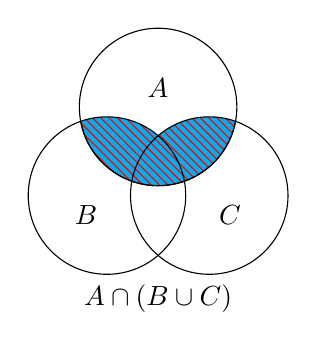
\begin{tikzpicture}
    \begin{scope}
        \clip \firstcircle;
        \fill[cyan] \secondcircle;
        \fill[cyan] \thirdcircle;
    \end{scope}
    \begin{scope}
        \clip \secondcircle \thirdcircle;
        \draw[pattern=north west lines, pattern color=red] \firstcircle;
    \end{scope}
    \draw \firstcircle node[text=black,above] {$A$};
    \draw \secondcircle node [text=black,below left] {$B$};
    \draw \thirdcircle node [text=black,below right] {$C$};
    \node[below] at (current bounding box.south) {$A \cap \left(B \cup C\right)$};
\end{tikzpicture}

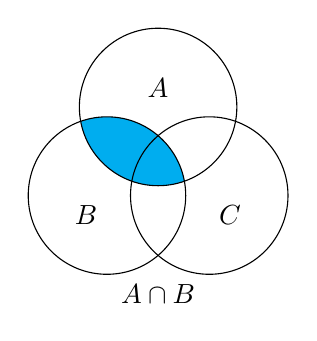
\begin{tikzpicture}
    \begin{scope}
        \clip \firstcircle;
        \fill[cyan] \secondcircle;
    \end{scope}
    \draw \firstcircle node[text=black,above] {$A$};
    \draw \secondcircle node [text=black,below left] {$B$};
    \draw \thirdcircle node [text=black,below right] {$C$};
    \node[below] at (current bounding box.south) {$A \cap B$};
\end{tikzpicture}

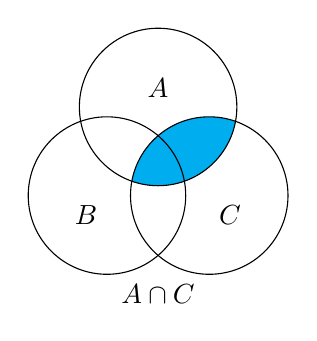
\begin{tikzpicture}
    \begin{scope}
        \clip \firstcircle;
        \fill[cyan] \thirdcircle;
    \end{scope}
    \draw \firstcircle node[text=black,above] {$A$};
    \draw \secondcircle node [text=black,below left] {$B$};
    \draw \thirdcircle node [text=black,below right] {$C$};
    \node[below] at (current bounding box.south) {$A \cap C$};
\end{tikzpicture}

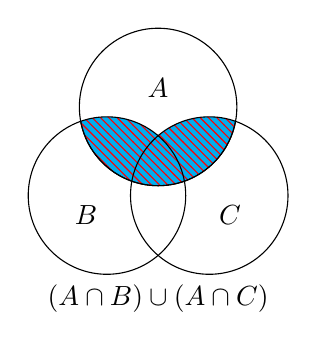
\begin{tikzpicture}
    \begin{scope}
        \clip \firstcircle;
        \fill[cyan] \secondcircle;
        \fill[cyan] \thirdcircle;
    \end{scope}
    \begin{scope}
        \clip \secondcircle \thirdcircle;
        \draw[pattern=north west lines, pattern color=red] \firstcircle;
    \end{scope}
    \draw \firstcircle node[text=black,above] {$A$};
    \draw \secondcircle node [text=black,below left] {$B$};
    \draw \thirdcircle node [text=black,below right] {$C$};
    \node[below] at (current bounding box.south) {$\left(A \cap B\right) \cup \left(A \cap C\right)$};
\end{tikzpicture}

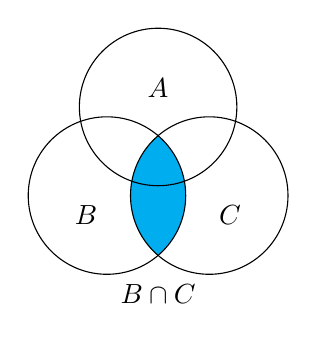
\begin{tikzpicture}
    \begin{scope}
        \clip \secondcircle;
        \fill[cyan] \thirdcircle;
    \end{scope}
    \draw \firstcircle node[text=black,above] {$A$};
    \draw \secondcircle node [text=black,below left] {$B$};
    \draw \thirdcircle node [text=black,below right] {$C$};
    \node[below] at (current bounding box.south) {$B \cap C$};
\end{tikzpicture}

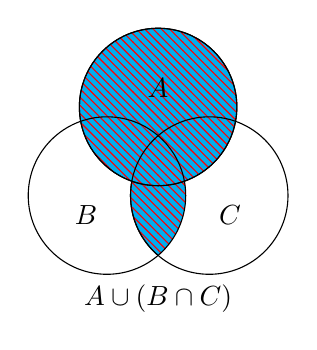
\begin{tikzpicture}
    \begin{scope}
        \clip \secondcircle;
        \fill[cyan] \thirdcircle;
        \draw[pattern=north west lines, pattern color=red] \thirdcircle;
    \end{scope}
    \fill[cyan] \firstcircle;
    \draw[pattern=north west lines, pattern color=red] \firstcircle;
    \draw \firstcircle node[text=black,above] {$A$};
    \draw \secondcircle node [text=black,below left] {$B$};
    \draw \thirdcircle node [text=black,below right] {$C$};
    \node[below] at (current bounding box.south) {$A \cup \left(B \cap C\right)$};
\end{tikzpicture}

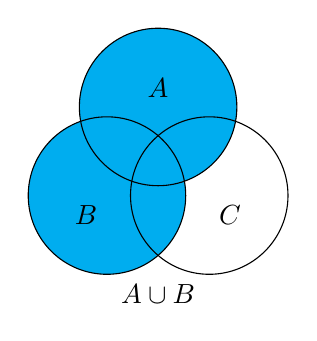
\begin{tikzpicture}
    \fill[cyan] \firstcircle;
    \fill[cyan] \secondcircle;
    \draw \firstcircle node[text=black,above] {$A$};
    \draw \secondcircle node [text=black,below left] {$B$};
    \draw \thirdcircle node [text=black,below right] {$C$};
    \node[below] at (current bounding box.south) {$A \cup B$};
\end{tikzpicture}

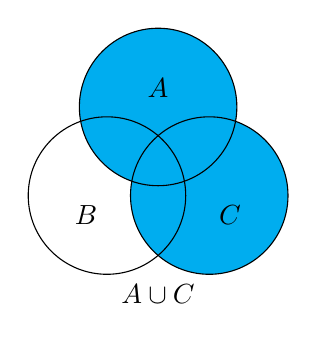
\begin{tikzpicture}
    \fill[cyan] \firstcircle;
    \fill[cyan] \thirdcircle;
    \draw \firstcircle node[text=black,above] {$A$};
    \draw \secondcircle node [text=black,below left] {$B$};
    \draw \thirdcircle node [text=black,below right] {$C$};
    \node[below] at (current bounding box.south) {$A \cup C$};
\end{tikzpicture}


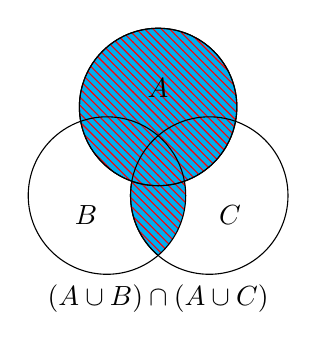
\begin{tikzpicture}
    \begin{scope}
        \clip \secondcircle;
        \fill[cyan] \thirdcircle;
        \draw[pattern=north west lines, pattern color=red] \thirdcircle;
    \end{scope}
    \fill[cyan] \firstcircle;
    \draw[pattern=north west lines, pattern color=red] \firstcircle;
    \draw \firstcircle node[text=black,above] {$A$};
    \draw \secondcircle node [text=black,below left] {$B$};
    \draw \thirdcircle node [text=black,below right] {$C$};
    \node[below] at (current bounding box.south) {$\left(A \cup B\right) \cap \left(A \cup C\right)$};
\end{tikzpicture}

\section*{3 Integration in the Complex Plane}
\subsection*{3.1 Path Integrals}



\end{document}